\section{Memory Decoding}
\label{sec:memory-decoding}

In addition to requiring storage components in a memory unit, there is a need for decoding circuits to select the memory word specified by the input address.

\subsection{Internal Construction}
\label{subsec:internal-construction}

The internal construction of a RAM of $m$ words and $n$ bits per word consists of $m \times n$ binary storage cells and associated decoding circuits for selecting individual words. The binary storage cell is the basic building block of a memory unit. The equivalent logic of a binary cell that stores one bit of information is shown in Fig. 5.
\begin{figure}[H]
  \centering
  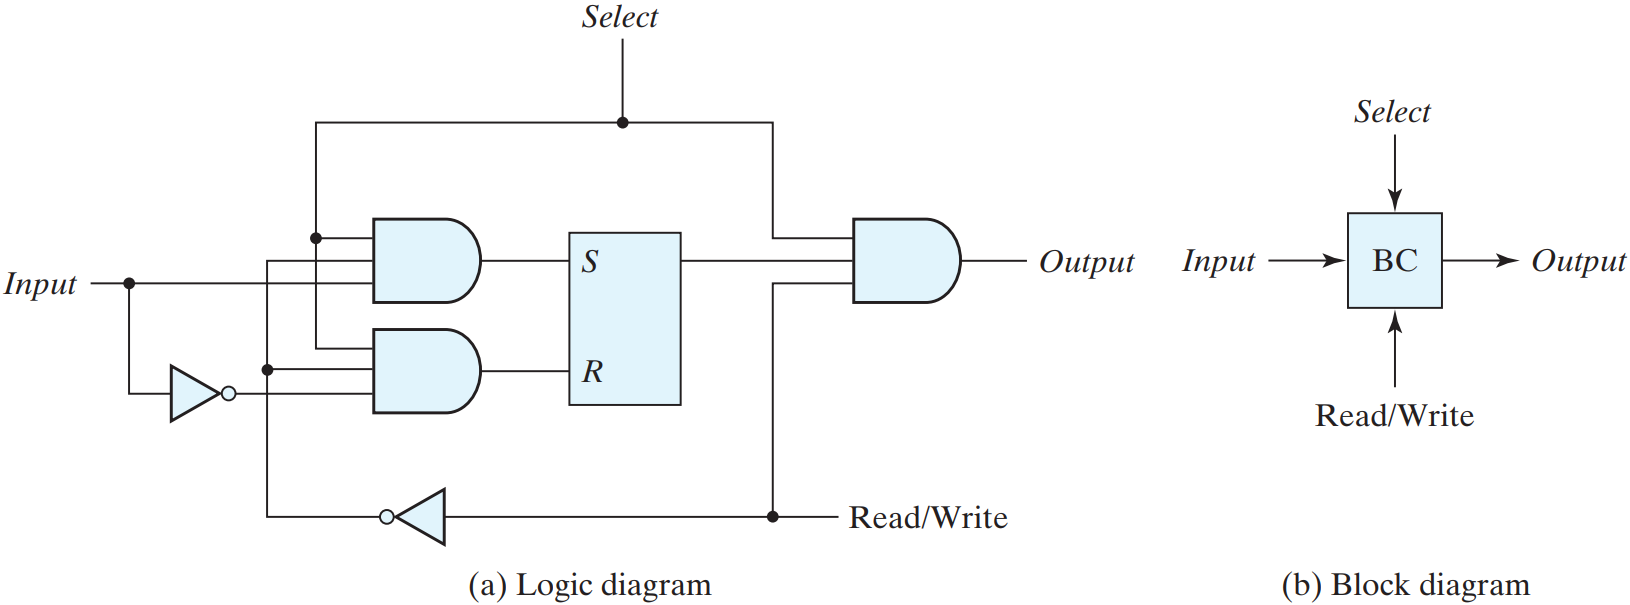
\includegraphics[width=\linewidth]{img/fig-7.5.png}
  \caption{Memory cell}
  \label{fig:7.5}
\end{figure}

Actually, the cell is an electronic circuit with \textit{four to six transistors}. Nevertheless, it is possible and convenient to model it in terms of logic symbols. A binary storage cell must be very small in order to be able to pack as many cells as possible in the small area available in the integrated circuit chip. 

The binary cell stores one bit in its internal latch. The select input enables the cell for reading or writing, and the read/write input determines the operation of the cell when it is selected.
\begin{itemize}
  \item \textit{Read}: A 1 in the read/write input provides the read operation by forming a path from the latch to the output terminal.
  \item \textit{Write}: A 0 in the read/write input provides the write operation by forming a path from the input terminal to the latch.
\end{itemize}

The logical construction of a small RAM is shown in Fig. 6. This RAM consists of four words of four bits each and has a total of 16 binary cells. The small blocks labeled BC represent the binary cell with its three inputs and one output, as specified in Fig. 5(b). 

A memory with four words needs two address lines. The two address inputs go through a $2 \times 4$ decoder to select one of the four words. The decoder is enabled with the memory enable input. When the memory enable is 0, all outputs of the decoder are 0 and none of the memory words are selected. With the memory select at 1, one of the four words is selected, dictated by the value in the two address lines. Once a word has been selected, the read/write input determines the operation.

\end{multicols*}

\begin{figure}[H]
  \centering
  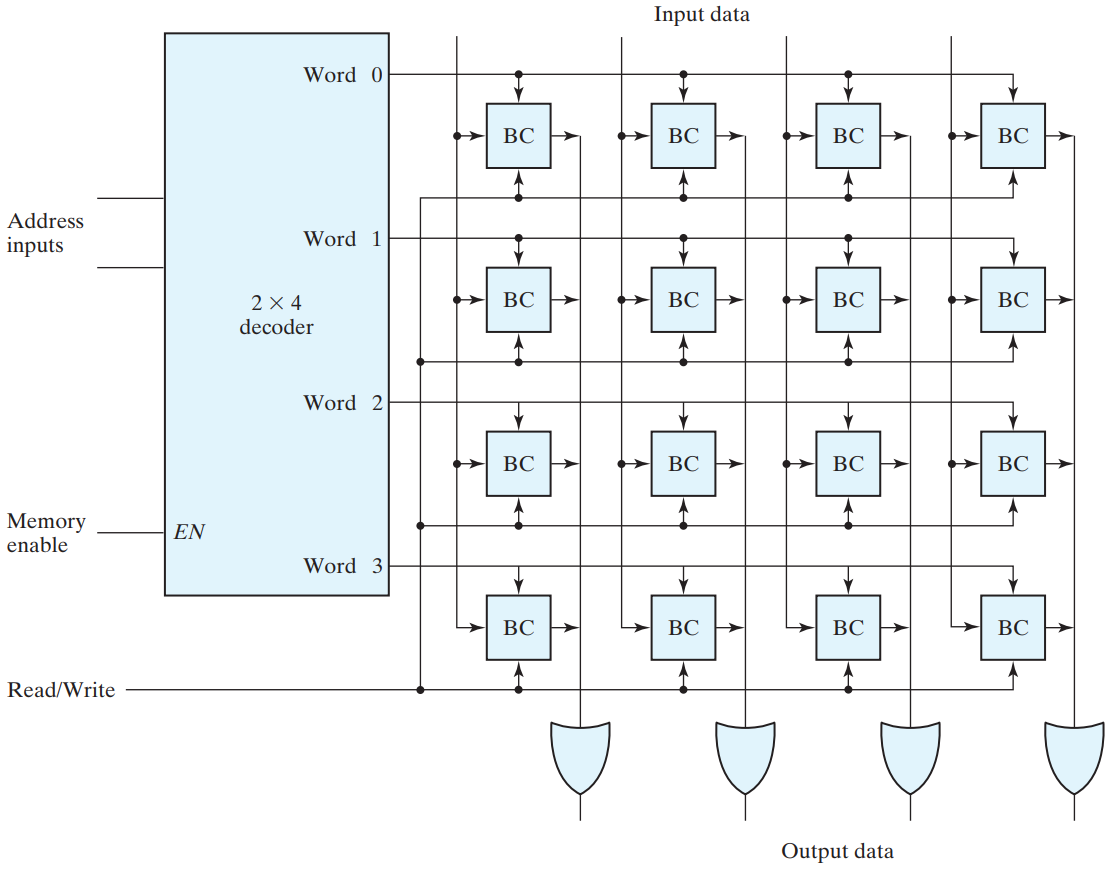
\includegraphics[width=\linewidth]{img/fig-7.6.png}
  \caption{Diagram of a $4 \times 4$ RAM}
  \label{fig:7.6}
\end{figure}

\begin{multicols}{2}
\setlength{\columnsep}{1.5cm}
\setlength{\columnseprule}{0.2pt}

\begin{itemize}
  \item During the read operation, the four bits of the selected word go through OR gates to the output terminals.
  \item During the write operation, the data available in the input lines are transferred into the four binary cells of the selected word.
\end{itemize}

The binary cells that are not selected are disabled, and their previous binary values remain unchanged. When the memory select input that goes into the decoder is equal to 0, none of the words are selected and the contents of all cells remain unchanged regardless of the value of the read/write input.

A memory with $2^k$ words of $n$ bits per word requires $k$ address lines that go into a $k \times 2^k$ decoder. Each one of the decoder outputs selects one word of $n$ bits for reading or writing.

\vspace*{\fill}
\columnbreak

\subsection{Coincident Decoding}
\label{subsec:coincident-decoding}

A decoder with $k$ inputs and $2^k$ outputs requires $2^k$ AND gates with $k$ inputs per gate. The total number of gates and the number of inputs per gate can be reduced by employing two decoders in a two-dimensional selection scheme. The basic idea in two-dimensional decoding is to arrange the memory cells in an array that is close as possible to square. In this configuration, two $k/2$-input decoders are used instead of one $k$-input decoder. One decoder performs the row selection and the other the column selection in a two-dimensional matrix configuration.

The two-dimensional selection pattern is demonstrated in Fig. 7 for a 1K-word memory. Instead of using a single $10 \times 1,024$ decoder, we use two $5 \times 32$ decoders. With the single decoder, we would need 1,024 AND gates with 10 inputs in each. In the two-decoder case, we need 64 AND gates with 5 inputs in each. The five most significant bits of the address go to input $X$ and the five least significant bits go to input $Y$.

Each word within the memory array is selected by the coincidence of one $X$ line and one $Y$ line. Thus, each word in memory is selected by the coincidence between 1 of 32 rows and 1 of 32 columns, for a total of 1,024 words. Note that each intersection represents a word that may have any number of bits.
\end{multicols}

\begin{figure}[H]
  \centering
  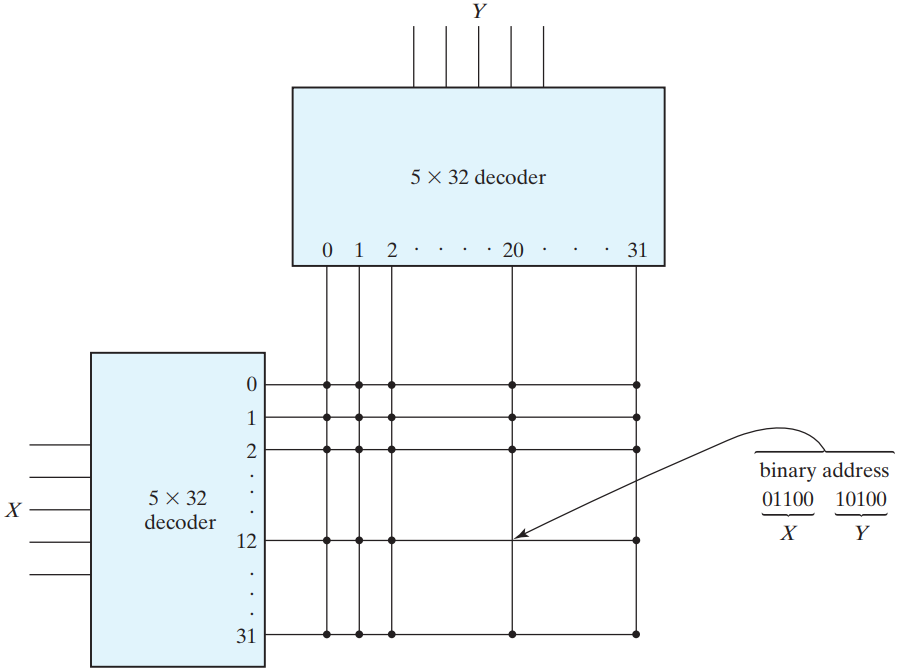
\includegraphics[width=\linewidth]{img/fig-7.7.png}
  \caption{Two-dimensional decoding structure for a 1K-word memory}
  \label{fig:7.7}
\end{figure}

\begin{multicols}{2}
\setlength{\columnsep}{1.5cm}
\setlength{\columnseprule}{0.2pt}

\subsection{Address Multiplexing}
\label{subsec:address-multiplexing}

The SRAM memory cell modeled in Fig. 5 typically contains six transistors. In order to build memories with higher density, it is necessary to reduce the number of transistors in a cell. The DRAM cell contains a single MOS transistor and a capacitor. The charge stored on the capacitor discharges with time, and the memory cells must be periodically recharged by refreshing the memory. 

Because of their simple cell structure, \textit{DRAMs typically have four times the density of SRAMs}. This allows four times as much memory capacity to be placed on a given size of chip. The cost per bit of DRAM storage is three to four times less than that of SRAM storage. A further (operational) cost savings is realized because of the lower power requirement of DRAM cells. 

These advantages make DRAM the preferred technology for large memories in personal digital computers. DRAM chips are available in capacities from 64K to 512M bits. Most DRAMs have a 1-bit word size, so several chips have to be combined to produce a larger word size.

\vspace*{\fill}
\columnbreak

Because of their large capacity, the address decoding of DRAMs is arranged in a two-dimensional array, and larger memories often have multiple arrays. To reduce the number of pins in the IC package, designers utilize address multiplexing whereby one set of address input pins accommodates the address components. In a two-dimensional array, the address is applied in two parts at different times, with the row address first and the column address second. Since the same set of pins is used for both parts of the address, the size of the package is decreased significantly.

We will use a 64K-word memory to illustrate the address-multiplexing idea. A diagram of the decoding configuration is shown in Fig. 8. The memory consists of a two-dimensional array of cells arranged into 256 rows by 256 columns, for a total of $2^8 \times 2^8 = 2^{16} = 64K$ words. There is a single data input line, a single data output line, and a read/write control, as well as an eight-bit address input and two address strobes, the latter included for enabling the row and column address into their respective registers. The row address strobe (RAS) enables the eight-bit row register, and the column address strobe (CAS) enables the eight-bit column register. The bar on top of the name of the strobe symbol indicates that the registers are enabled on the zero level of the signal.

\end{multicols}

\begin{figure}[H]
  \centering
  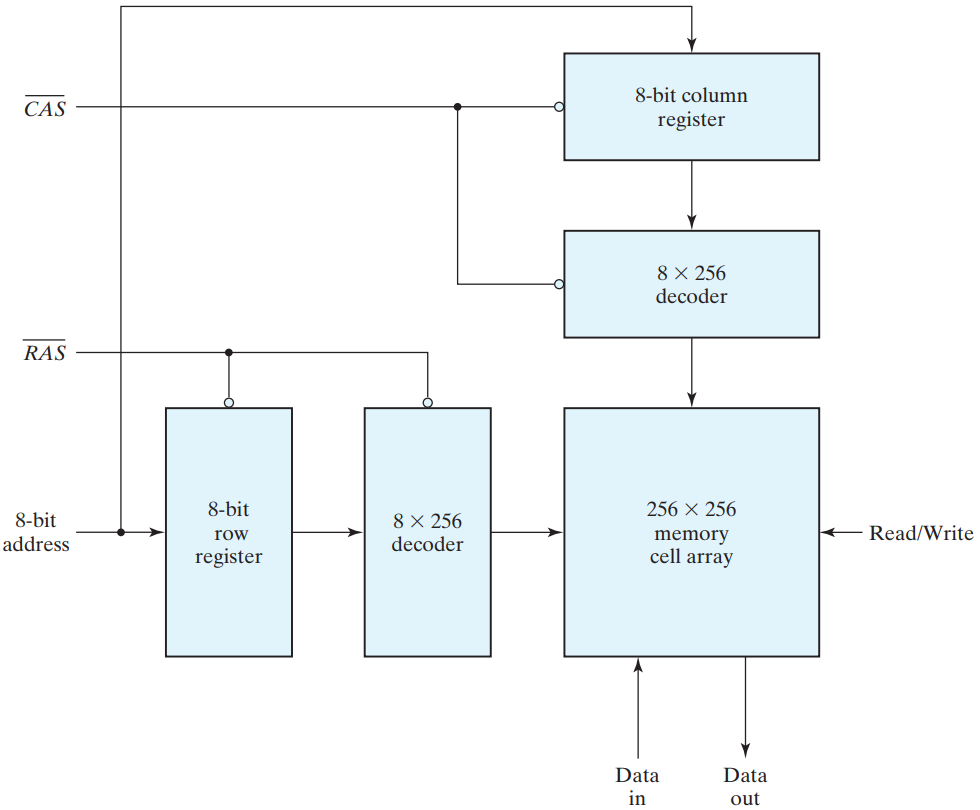
\includegraphics[width=\linewidth]{img/fig-7.8.png}
  \caption{Address multiplexing for a 64K DRAM}
  \label{fig:7.8}
\end{figure}

\begin{multicols}{2}
\setlength{\columnsep}{1.5cm}
\setlength{\columnseprule}{0.2pt}